% region Filename parsing.
% Provides macros manipulating strings of tokens.
\RequirePackage{xstring}

% Store the jobname as a string with category 11 characters.
\edef\normaljobname{\expandafter\scantokens\expandafter{\jobname\noexpand}}
\StrBetween{\normaljobname}{hw-}{-q}[\homeworknumber]
\StrBehind{\normaljobname}{-q-}[\questionnumber]
% endregion Filename parsing.

\documentclass[
  coursecode={MTHE 418},
  assignmentname={Homework \homeworknumber},
  studentnumber=20053722,
  name={Bryan Hoang},
  draft,
  % final,
]{
  ltxanswer%
}

\usepackage{bch-style}

\usepackage{dsfont}
\usepackage[margin=2cm]{geometry}
\usepackage{pgfplots}
\usetikzlibrary{calc,intersections}
\usepgfplotslibrary{groupplots}
\pgfplotsset{compat=1.16}
\newcommand{\MyGroupPlot}{
    \edef\temp{\noexpand\nextgroupplot[title={$A=\mya,B=\myb$},xmin=\myxmin-0.5,xmax=\myxmin+\myd+0.5]
      \noexpand\addplot [thick,domain=\myxmin:\myxmin+\myd,smooth] {ysol(x,\mya,\myb)};
      \noexpand\addplot [thick,domain=\myxmin:\myxmin+\myd,smooth] {-ysol(x,\mya,\myb)};
      \noexpand\addplot [smooth,thick] coordinates {({\myxmin+min(\myd,1)/20},{-ysol(\myxmin+min(\myd,1)/20,\mya,\myb)})
        ({\myxmin+min(\myd,1)/40},{-ysol(\myxmin+min(\myd,1)/40,\mya,\myb)})
        (\myxmin,0) ({\myxmin+min(\myd,1)/40},{ysol(\myxmin+min(\myd,1)/40,\mya,\myb)})
        ({\myxmin+min(\myd,1)/20},{ysol(\myxmin+min(\myd,1)/20,\mya,\myb)})};}
    \temp
}

\begin{document}
  \begin{questions}
    \setcounter{question}{\questionnumber}
    \addtocounter{question}{-1}
    \question[10]\
    \begin{solution}
      \begin{answerfigure}
        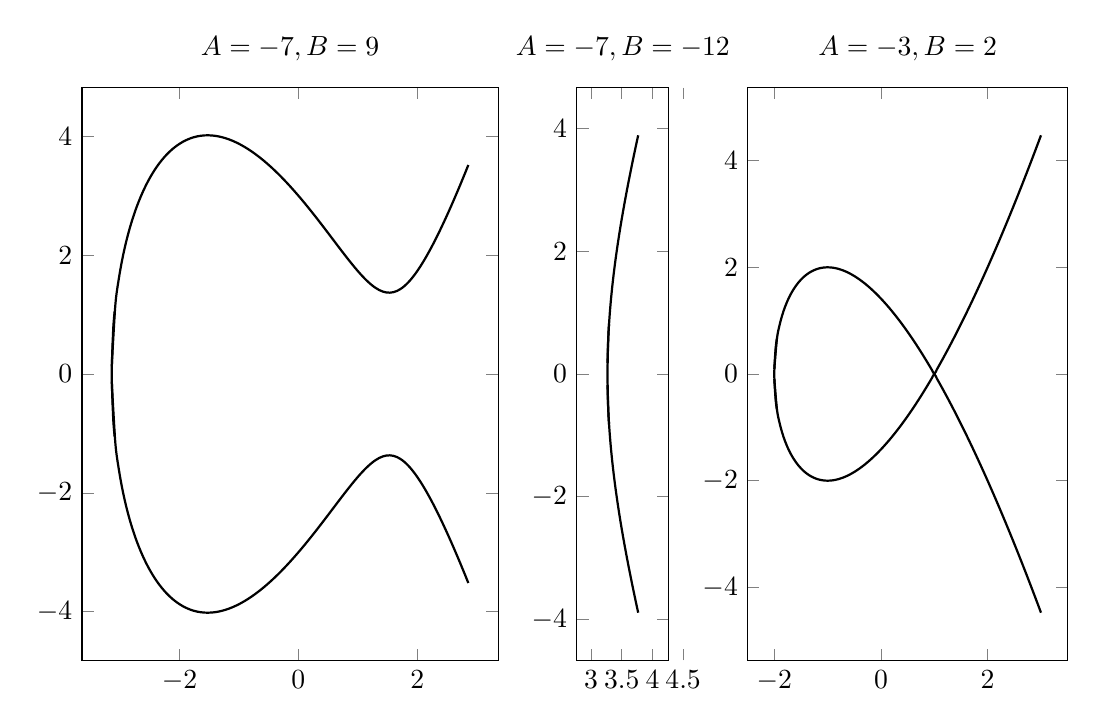
\begin{tikzpicture}[declare function={xnod(\a,\b)=0.001+%
                (-2*pow(3,1/3)*\a + pow(2,1/3)*
                pow(abs(-9*\b + sqrt(12*pow(\a,3) + 81*pow(\b,2))),2/3))/%
                (pow(6,2/3)*sign(-9*\b + sqrt(12*pow(\a,3) +  81*pow(\b,2)))*%
                pow(abs(-9*\b + sqrt(12*pow(\a,3) +  81*pow(\b,2))),1/3));
                ysol(\x,\a,\b)=sqrt((\x*\x*\x+\a*\x+\b));}]
          \begin{groupplot}[group style={group size=3 by 1},
              scale only axis,
              samples=101,
              % use same unit vectors on the axis
              axis equal image=true,
            ]
            \edef\mya{-7}
            \edef\myb{9}
            \edef\myd{6}
            \pgfmathsetmacro{\myxmin}{xnod(\mya,\myb)}
            \MyGroupPlot
            \edef\mya{-7}
            \edef\myb{-12}
            \edef\myd{0.5}
            \pgfmathsetmacro{\myxmin}{xnod(\mya,\myb)}
            \MyGroupPlot
            \edef\mya{-3}
            \edef\myb{2}
            \edef\myd{5}
            \pgfmathsetmacro{\myxmin}{xnod(\mya,\myb)}
            \MyGroupPlot
          \end{groupplot}
        \end{tikzpicture}
        \caption{A group plot of the elliptic curves for parts (b), (c), and (d) respectively.}
        \label{fig:elliptic}
      \end{answerfigure}
    \end{solution}
  \end{questions}
\end{document}
